\chapter{Theoretical Background}
\label{chap:theoretical-background}
Since the application's core is sentiment analysis, it is necessary to define the basic concepts. \textcolor{lightgray}{Lorem ipsum dolor sit amet, consectetur adipiscing elit. Sed non risus. Suspendisse lectus tortor, dignissim sit amet, adipiscing nec, ultricies sed, dolor. Lorem ipsum dolor sit amet, consectetur adipiscing elit. Sed non risus. Suspendisse lectus tortor, dignissim sit amet, adipiscing nec, ultricies sed, dolor. Lorem ipsum dolor sit amet, consectetur adipiscing elit. Sed non risus. Suspendisse lectus tortor, dignissim sit amet, adipiscing nec, ultricies sed, dolor. Lorem ipsum dolor sit amet, consectetur adipiscing elit. Sed non risus.}

\section{Sentiment Analysis Basics}
\label{sec:sentiment-analysis-basics}
Sentiment analysis or opinion mining is a subfield of \acrfull{nlp} that aims to identify and extract opinions and emotions from a text. The~goal is to determine the author's attitude towards a particular topic or the overall contextual polarity~of various document levels. We measure the text's polarity using a numerical scale ranging from -1 to 1. The low-end score of the scale signifies a negative sentiment, zero represents neutrality, and the high-end score indicates a positive sentiment. This scale effectively estimates the degree of negativity or positivity in the text's tone. 

The extraction of opinions and emotions has applications in various areas, from product reviews to political events. Hence, it is imperative to work in different domains (see \cite{PIRYANI2017122}). Because of cross-domain and cross-language, two of the most general issues in sentiment analysis, this thesis will focus only on the financial domain in English. Nevertheless, domain-specific sentiment analysis achieves remarkable accuracy while staying highly domain-sensitive, as shown in \parencite{saunders_2020}. To delve deeper into cross issues, \citeauthor{liu2022sentiment} provides further details in his book \parencite{liu2022sentiment}.

\subsection{Levels of Sentiment Analysis}
\label{subsec:levels-of-sentiment-analysis}
Sentiment analysis has been studied at several levels of granularity: Document-level, Sentence-level, Phrase-level, and Entity-level\footnote{Entities are sometimes referred to as targets, hence Target-level or Target-based sentiment analysis.}, as illustrated in Figure \ref{fig:sa-levels}.

\begin{figure}[H]
    \centering
    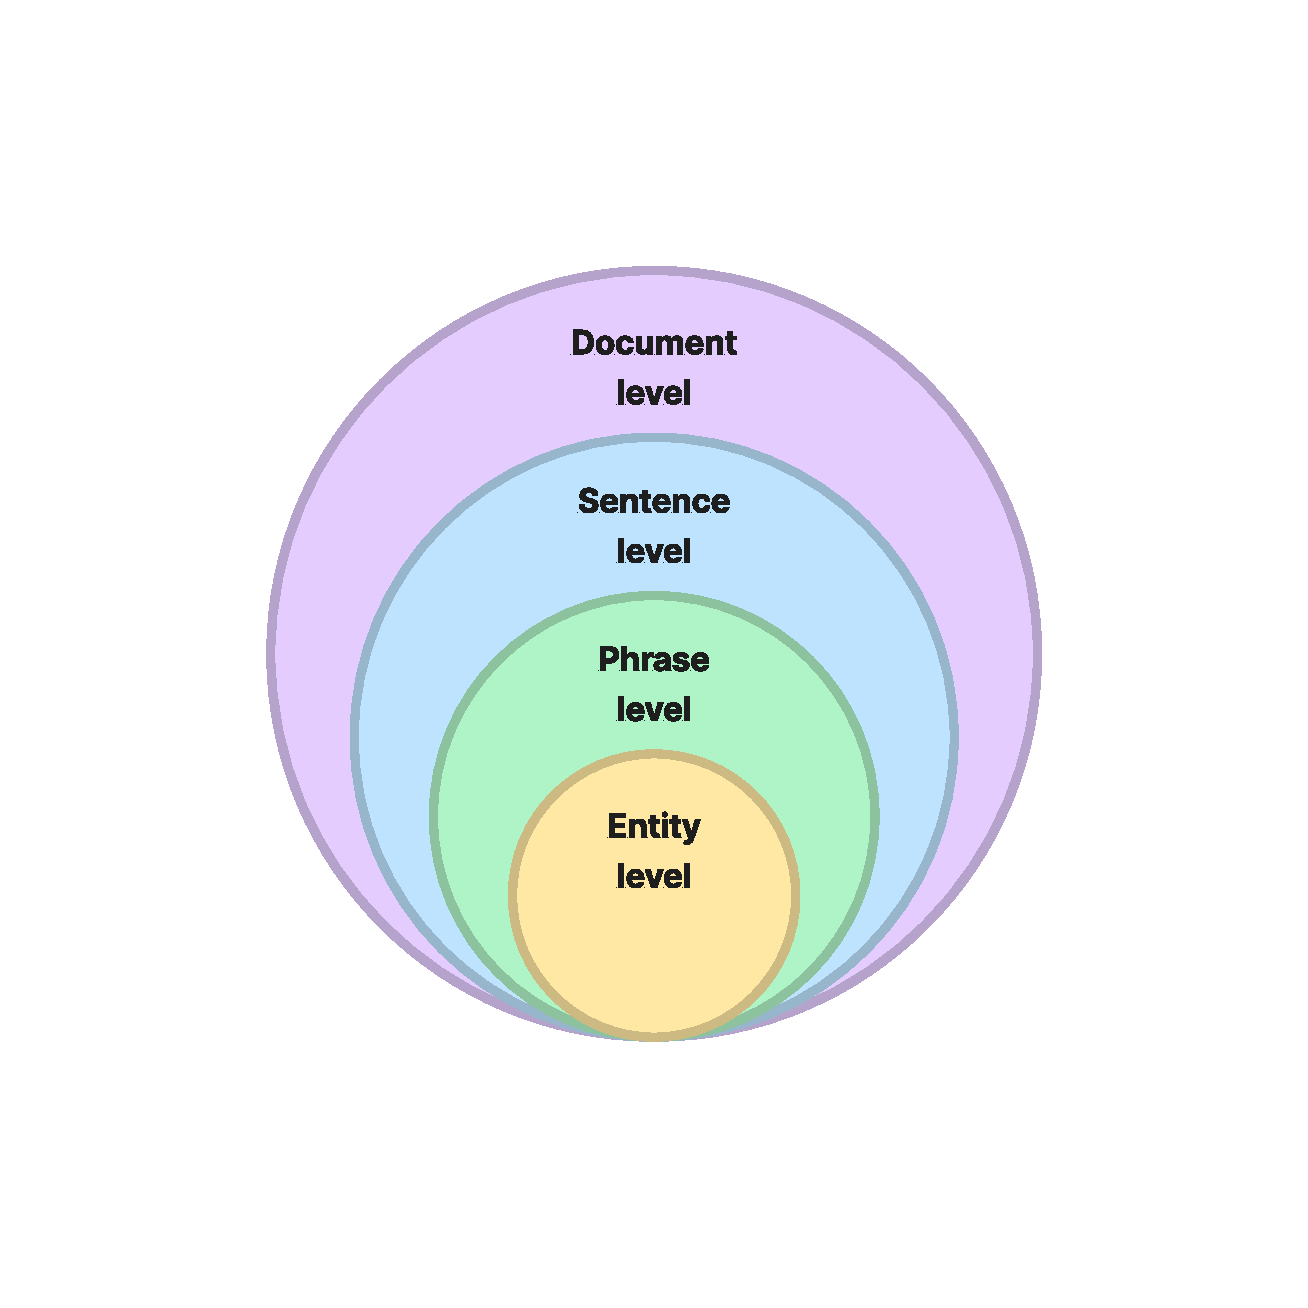
\includegraphics[width=0.5\textwidth]{img/sa-levels.pdf}
    \caption{Levels of sentiment analysis (inspired by \cite{Wankhade2022}).}
    \label{fig:sa-levels}
\end{figure}

\subsubsection*{Document-level}
\label{subsubsec:document-level}
%At the first level is document-level sentiment analysis. This level is the most straight.
Document-level sentiment analysis is the most straight level. The task is to determine the overall emotional context of the entire document, such as a chapter, article, or review, whether or not involving a study of entities or aspects. This level gives us a general assessment of whether the content is more likely to be positive, negative, or neutral. 

\subsubsection*{Sentence-level}
\label{subsubsec:sentence-level}
Sentiment analysis at the sentence level focuses on individual sentences within the text. We observe the polarity of each sentence autonomously, employing the same methodologies utilized at the document level but with an increased volume of training data and enhanced processing resources. This level is more challenging than the document level because it requires a more in-depth understanding of the text. 

\subsubsection*{Phrase-level}
\label{subsubsec:phrase-level}
Phrase-level sentiment analysis examines sentiment within smaller linguistic units such as phrases or sentence members. Thus, it can better reveal the emotional charge in specific parts of sentences.  Additionally, this level is more challenging than the sentence level because it requires a more detailed understanding of the text. 


\subsubsection*{Entity-level}
\label{subsubsec:entity-level}
%https://wandb.ai/madhana/Named_Entity_Recognition/reports/A-Beginner-s-Guide-to-Named-Entity-Recognition-NER---VmlldzozNjE2MzI1
The most elaborative level is entity-level sentiment analysis, where we study sentiment associated with specific entities mentioned in the text. This level provides a detailed look at the expressed polarity of certain products, individuals, or organisations. One of the main tasks in this scope is the named entity recognition, which will be discussed later.

\paragraph{}

Some researchers classify the last level as the aspect-level, as noted by \cite{Wankhade2022}, or a more detailed entity-level version called the feature-level proposed by \cite{Jenifer2017}. While both approaches aim to evaluate sentiment towards specific aspects, they differ in their task approach. Relationships between these levels are illustrated in Figure \ref{fig:entity-feature-aspect-level}.

In the first case, aspects are considered without directly mentioning entities in the text. We are not interested in the entities since the input textual data are commonly associated with them\footnote{Entities are not handled in this case, but we provide them here for a better understanding.}, such as reviews. The study conducted by \cites{Wang2019} analyzed sentiment at the aspect level within restaurant reviews. It primarily examines aspects such as food, price, service, and others. In~the feature-based approach, aspects are commonly associated with an entity's features by connecting the entity and its aspects in text. To illustrate, consider the sentence:\begin{quote}
    \textit{``The battery life of this phone is excellent, but the camera is not good.''}
\end{quote} At the feature level, we identify \textit{the battery life} and \textit{camera} as specific features of entity \textit{the phone}, allowing us to determine the polarity of each entity's feature.

\begin{figure}[H]
    \centering
    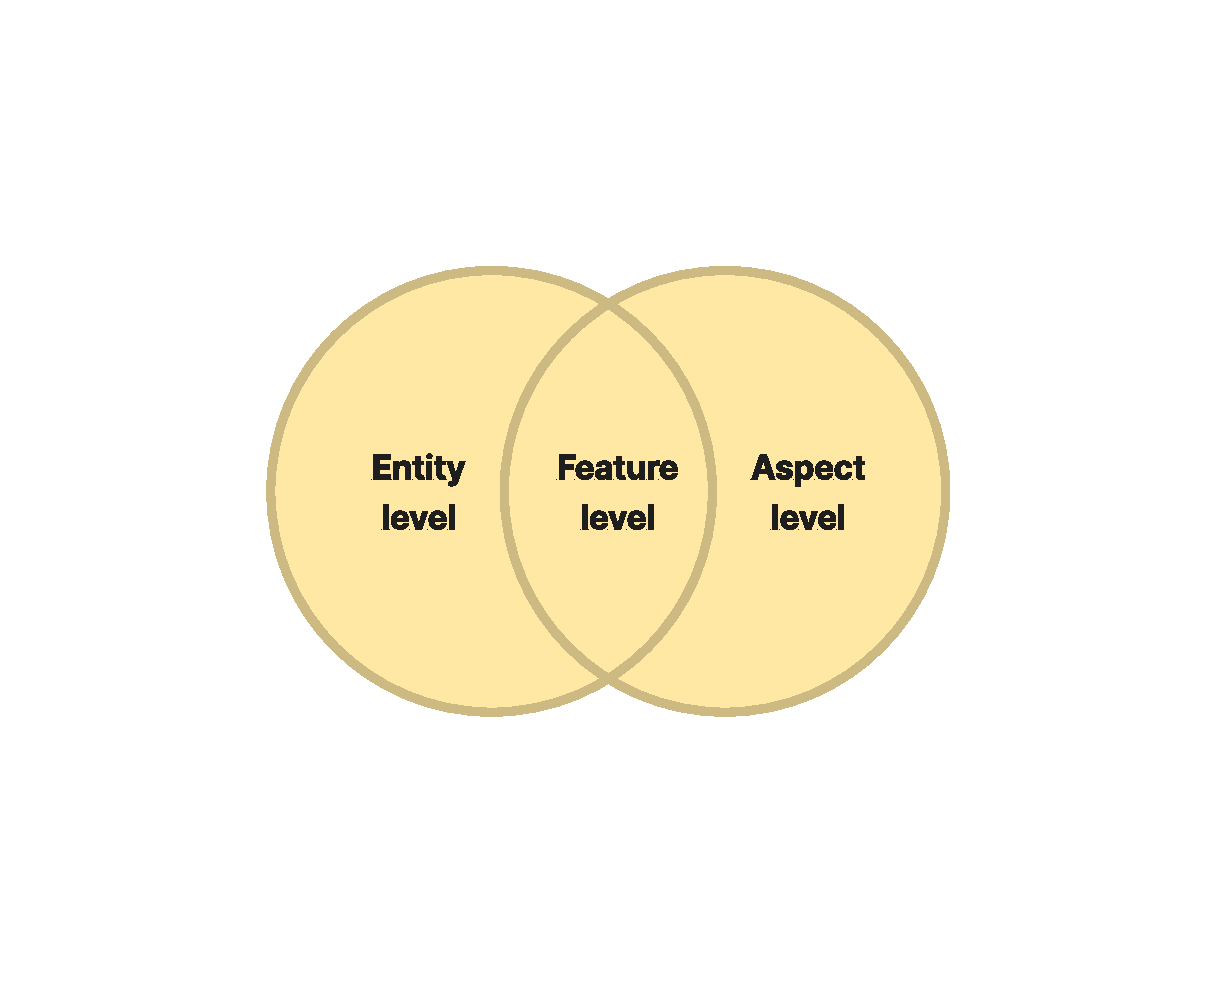
\includegraphics[width=0.5\textwidth]{img/entity-feature-aspect-level.pdf}
    \caption{Comprehensive overview of the last level.}
    \label{fig:entity-feature-aspect-level}
\end{figure}

% Každé rozdělení posledního levelu zkoumáme v rámci předešlých levelů. Toz namneá, že entity level zkoumáme v rámci document, sentence a nebo phrase. Opačně můžeme ale i nemusíme zkoumat document, sentence a nebo phrase v rámci entity levelu.

The term entity-level sentiment analysis is frequently employed in literature, and some studies consider it synonymous with targeted sentiment analysis, \linebreak as discussed \cite{ronningstad-etal-2022-entity} in the terminology review. For our purposes, entity-level sentiment analysis better captures the aggregate, document-wide approach, where a single entity can be associated with multiple targets in different sentences, discerning it from traditional target-level sentiment analysis. 

However, this thesis primarily focuses on entity-level sentiment analysis, excluding consideration of the entity's features. This decision is motivated by treating the mentioned companies in news articles as entities rather than delving into their specific aspects.\todo{TODO: Pokud nenarazím na článek, který by to vyvrátil. Navíc se zkoumáním aspektů by přibylo spousty práce.} Additionally, entity and aspect extraction as separate tasks are complex and challenging, given that the methods \textcolor{lightgray}{and facets} employed for recognition differ due to their distinct characteristics \parencite{Liu2015, Zhang2014}. 

\section{Named Entity Recognition}
\label{sec:named-entity-recognition}
% Good survey https://wandb.ai/madhana/Named_Entity_Recognition/reports/A-Beginner-s-Guide-to-Named-Entity-Recognition-NER---VmlldzozNjE2MzI1
% TODO Coding:
% - https://www.johnsnowlabs.com/rule-based-entity-recognition-with-spark-nlp/
% - https://bookdown.org/morleyjamesweston/MCM4TM/named-entity-recognition.html
Named entity recognition, or entity extraction, constitutes a fundamental component in \acrshort{nlp} dedicated to identifying and classifying proper nouns into predefined semantic classes. These classes are unlimited since entities could be anything we can categorize using a tag, including the names of organisations, people, places, or other available information from unstructured textual data such as time, quantity, and money expressions. Someone well-versed in data analysis must have contemplated the possibility that some sources provide data in which the names of organisations are directly associated with their unique tags in text, but this is not our case\todo{TODO: Vrátit se až budu mít všechny 3 zdroje a případně pozměnit na "né vždy náš případ."} (for more details, see Chapter \ref{chap:textual-data}). Understanding the importance of this task, we recognise its essential role in entity-level sentiment analysis, as it allows us to identify the emotion associated with specific entities mentioned in the text.

\begin{figure}[H]
    \centering
    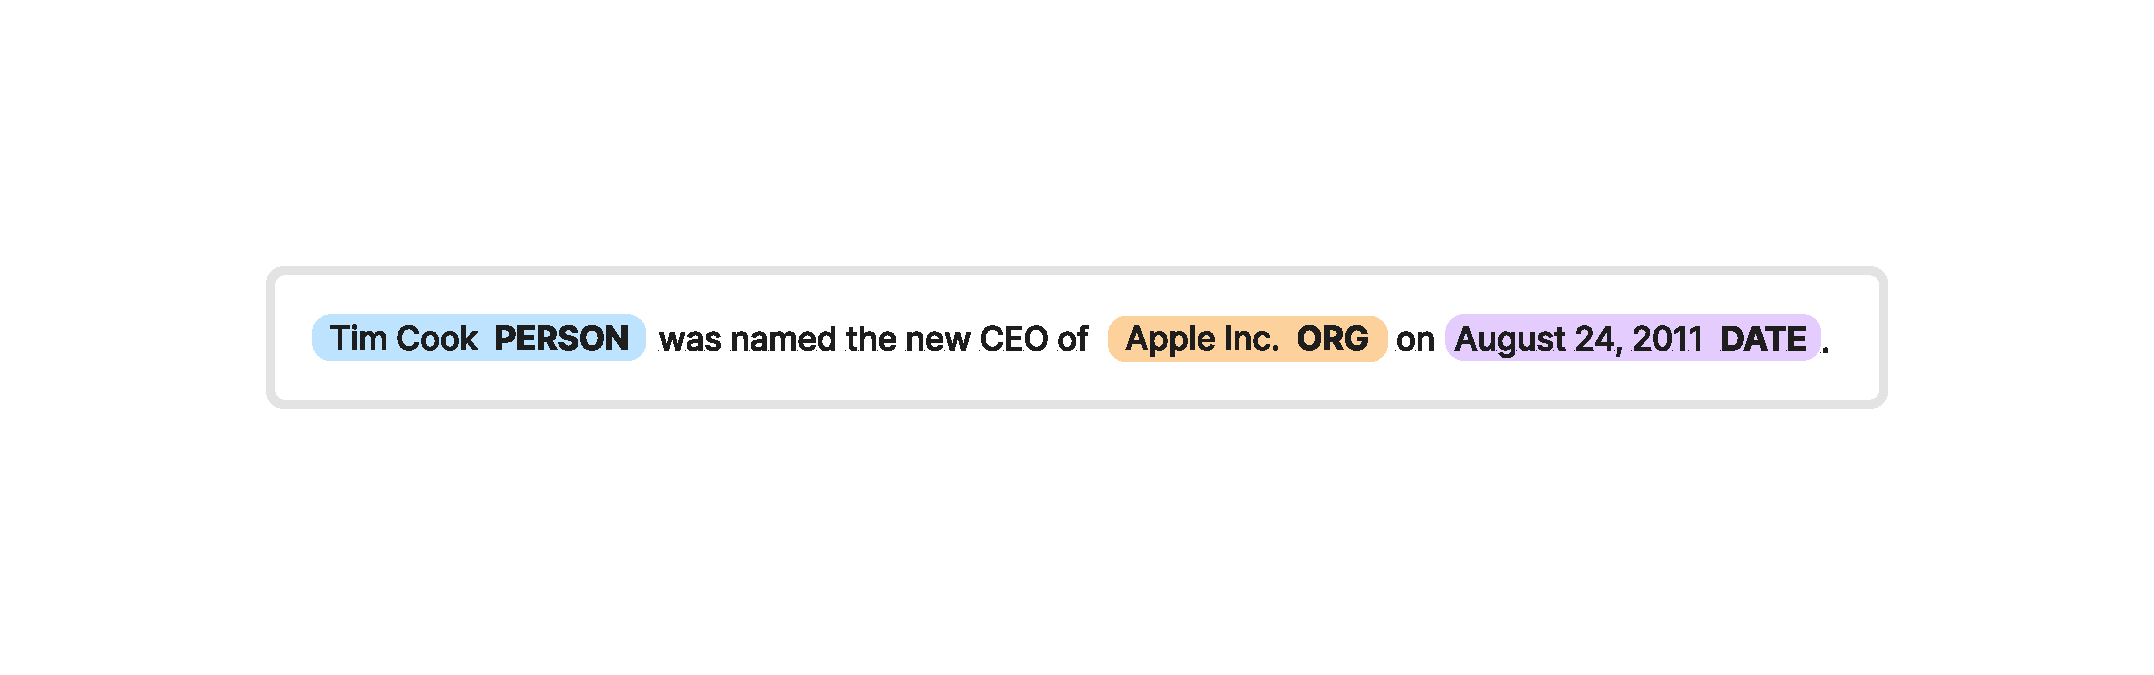
\includegraphics[width=\textwidth]{img/ner-theoretical-example.pdf}
    \caption{TODO: Named entities along with their associated label classes.}
    \label{fig:named-entity-recognition-theoretical-example}
\end{figure}

The example above illustrates that a single entity can contain more than one word. This challenge is addressed by token tagging formats outlined in the paper \parencite{ramshaw-marcus-1995-text}. Individual words are referred to as tokens. The formats describe the position of each token in a named entity, such as the \acrfull{bio} format, also known as the \acrfull{iob} format as well as other derived names like \acrfull{io} and \acrfull{bmewo}. These formats discharge us from the constraints of entities, which are hard-coded or unreliably specified by regular expressions.

\begin{figure}[H]
    \centering
    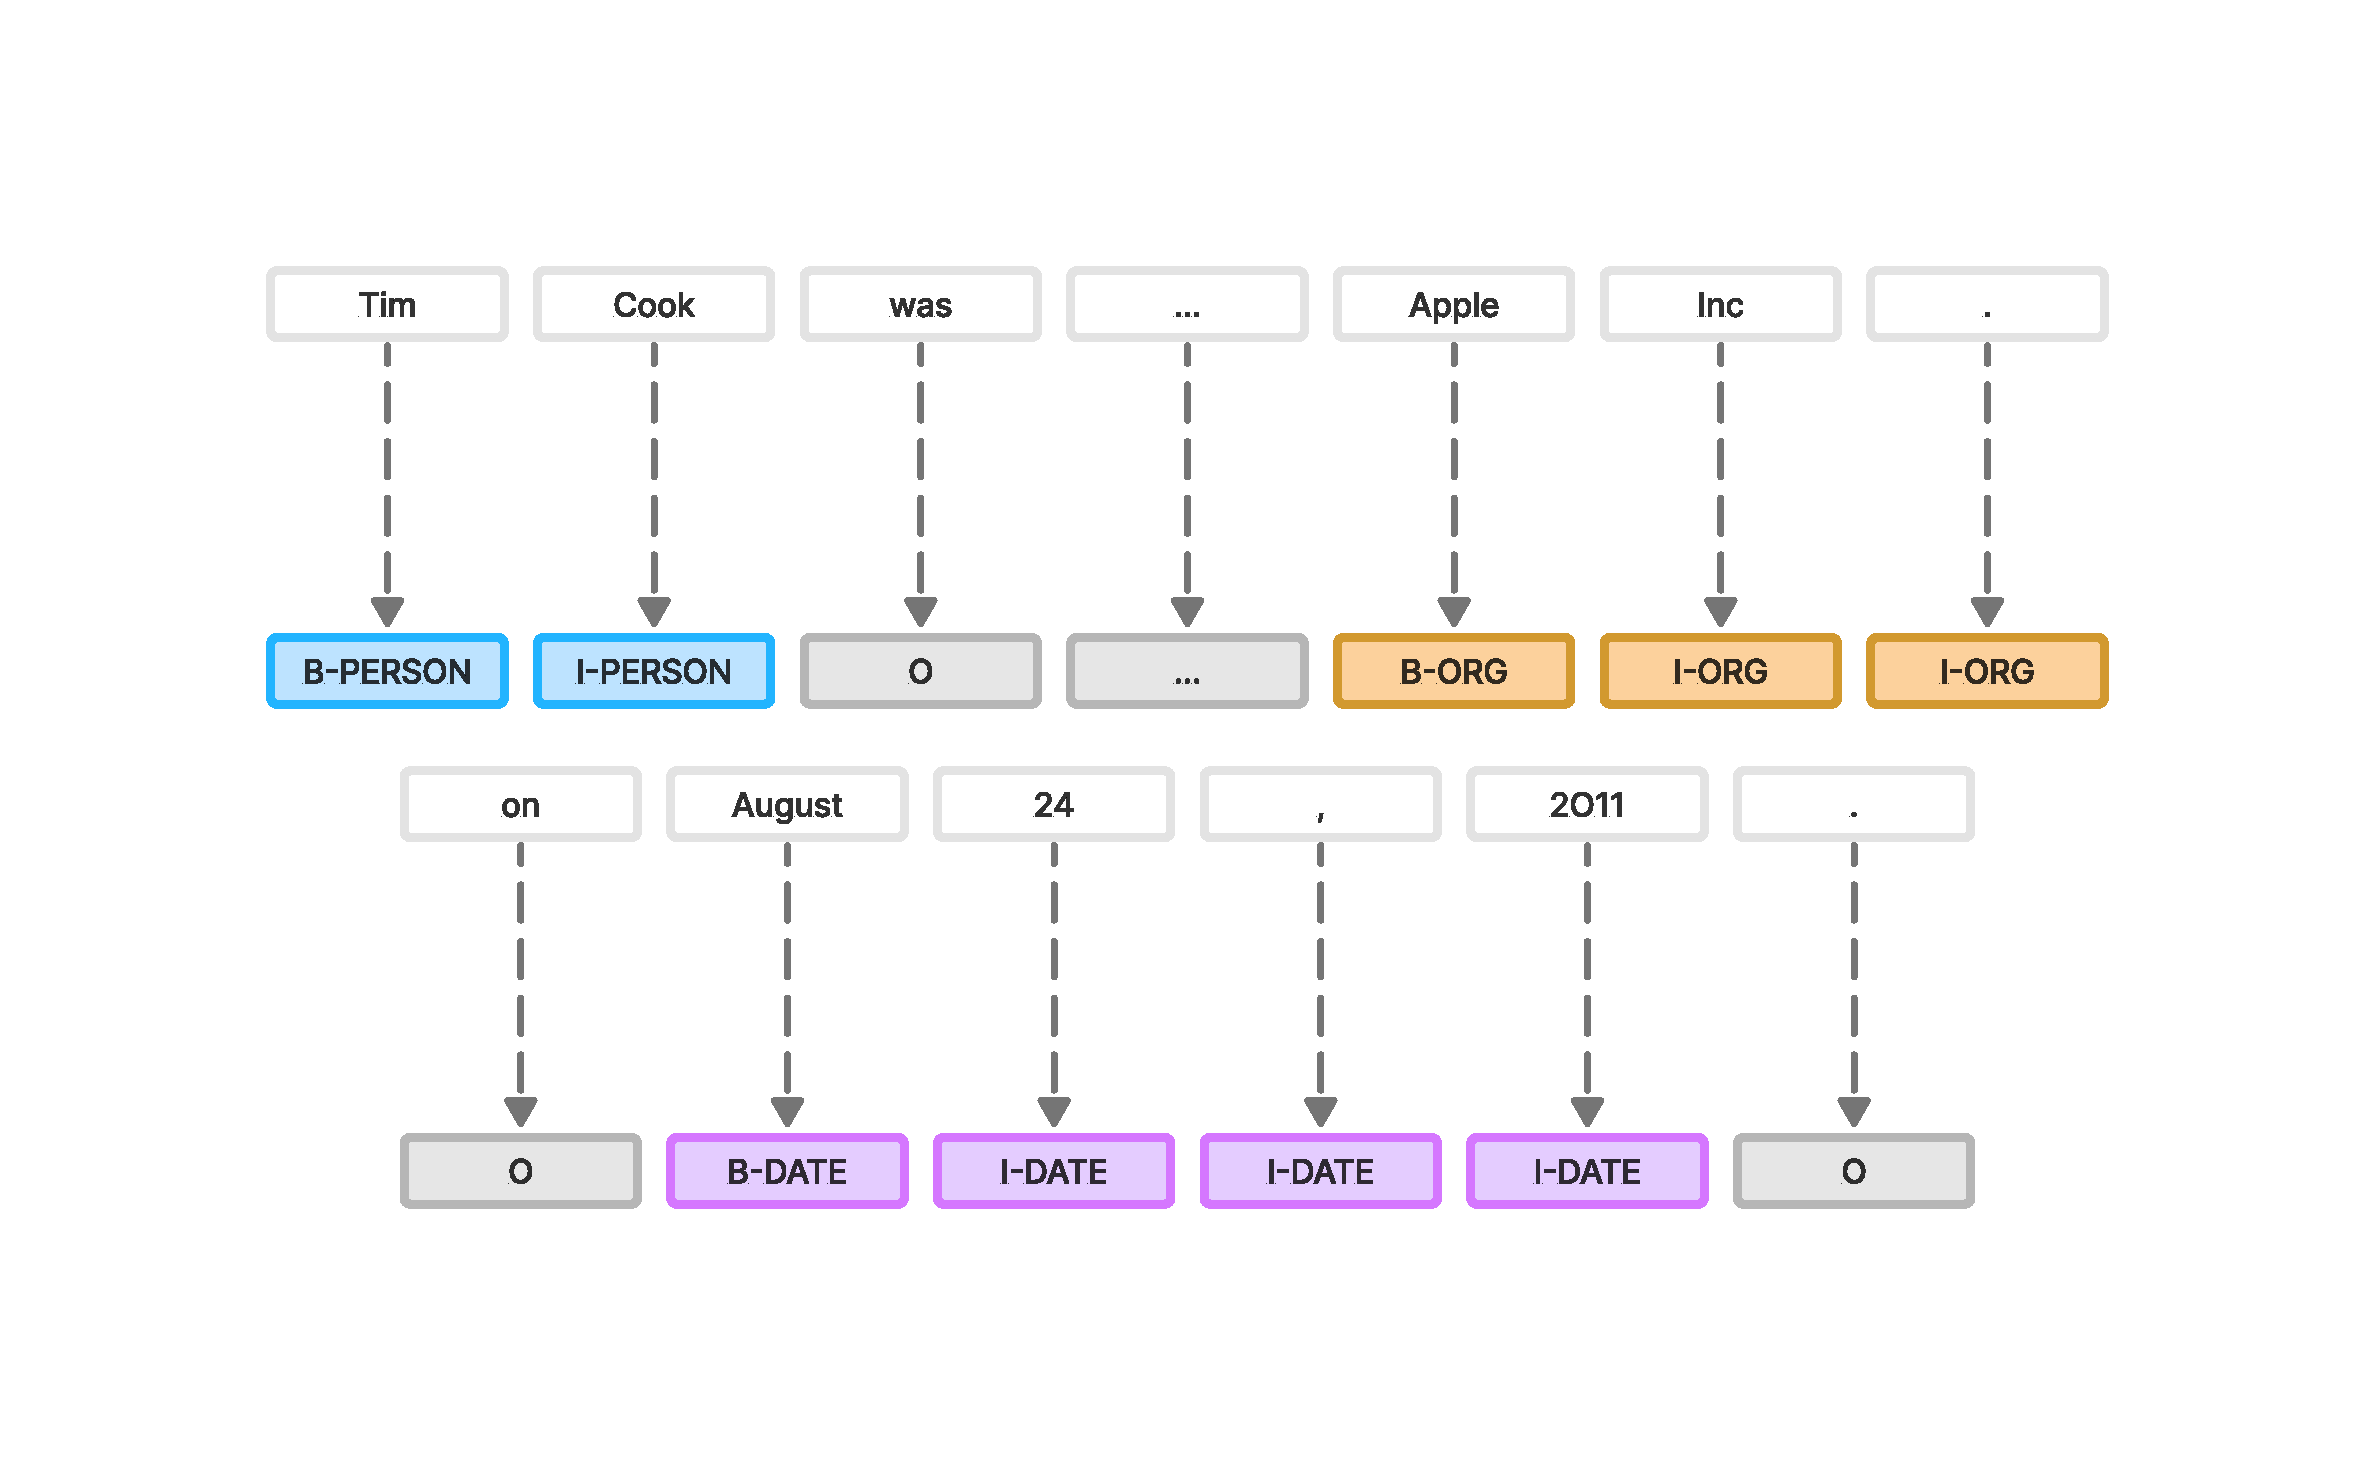
\includegraphics[width=\textwidth]{img/ner-theoretical-example-tags.pdf}
    \caption{TODO - \acrshort{bio}2 format.}
    \label{fig:named-entity-recognition-theoretical-example-tags}
\end{figure}

The tags that assign tokens to each entity class contain prefixes. The prefix I- indicates that the token is contained in the named entity, whereas O- indicates that the token is not contained in any named entity. The prefix B- is slightly more specific and indicates that the token is contained at the beginning of the named entity, followed immediately by a token not containing the O- prefix. A particular case of the \acrshort{bio} approach is the \acrshort{bio}2 format, denoting all tokens beginning with the prefix B-, regardless of whether a token with an O- prefix follows. A slightly more detailed approach is \acrshort{bmewo}, where the prefixes B- and O-, as in the previous ones, indicate the beginning and absence of the named entity occurrence, respectively. M- prefix symbolises the middle token between B- and E-, where the token with the prefix E- ends the named entity. Furthermore, the prefix W- indicates a single-token named entity. Table \ref{table:ner-theoretical-example-tags} below demonstrates how the mentioned sentence could be labeled with \acrshort{io}, \acrshort{bio}, \acrshort{bio}2, and \acrshort{bmewo} formats.
\begin{table}[ht]
    \centering
    \caption{TODO}
    \label{table:ner-theoretical-example-tags}
    %\renewcommand{\arraystretch}{1.1} 
    \begin{tabular}[t]{lllll}
        \hline
        &\multicolumn{4}{c}{Format}\\
        \cline{2-5}
        Token&IO&BIO&BIO2&BMEWO\\
        \hline
        Tim&I-PERSON&I-PERSON&B-PERSON&B-PERSON\\
        Cook&I-PERSON&I-PERSON&I-PERSON&E-PERSON\\
        was&O&O&O&O\\
        \dots&O&O&O&O\\
        Apple&I-ORG&I-ORG&B-ORG&B-ORG\\
        Inc&I-ORG&I-ORG&I-ORG&M-ORG\\
        .&I-ORG&I-ORG&I-ORG&E-ORG\\
        on&O&O&O&O\\
        August&I-DATE&I-DATE&B-DATE&B-DATE\\
        24&I-DATE&I-DATE&I-DATE&M-DATE\\
        ,&I-DATE&I-DATE&I-DATE&M-DATE\\
        2011&I-DATE&I-DATE&I-DATE&E-DATE\\
        .&O&O&O&O\\
        \hline
    \end{tabular}
\end{table}

%In a given text, there could be several mentions of separate entities, each possibly referred to directly and indirectly multiple times, with varying polarities. 
\subsection{Techniques}
\label{subsec:Techniques}
\todo{TODO: Posunout k obrázku.}
Approaches for entity extraction from unstructured data encompass a broad range of techniques, though they commonly converge into three principal categories. Specifically, the work \parencite{keraghel2024survey} classifies them in the following way: Knowledge-based, Feature engineering, and Deep learning, as illustrated in Figure \ref{fig:named-entity-recognition-methods} below.

\begin{figure}[H]
    \centering
    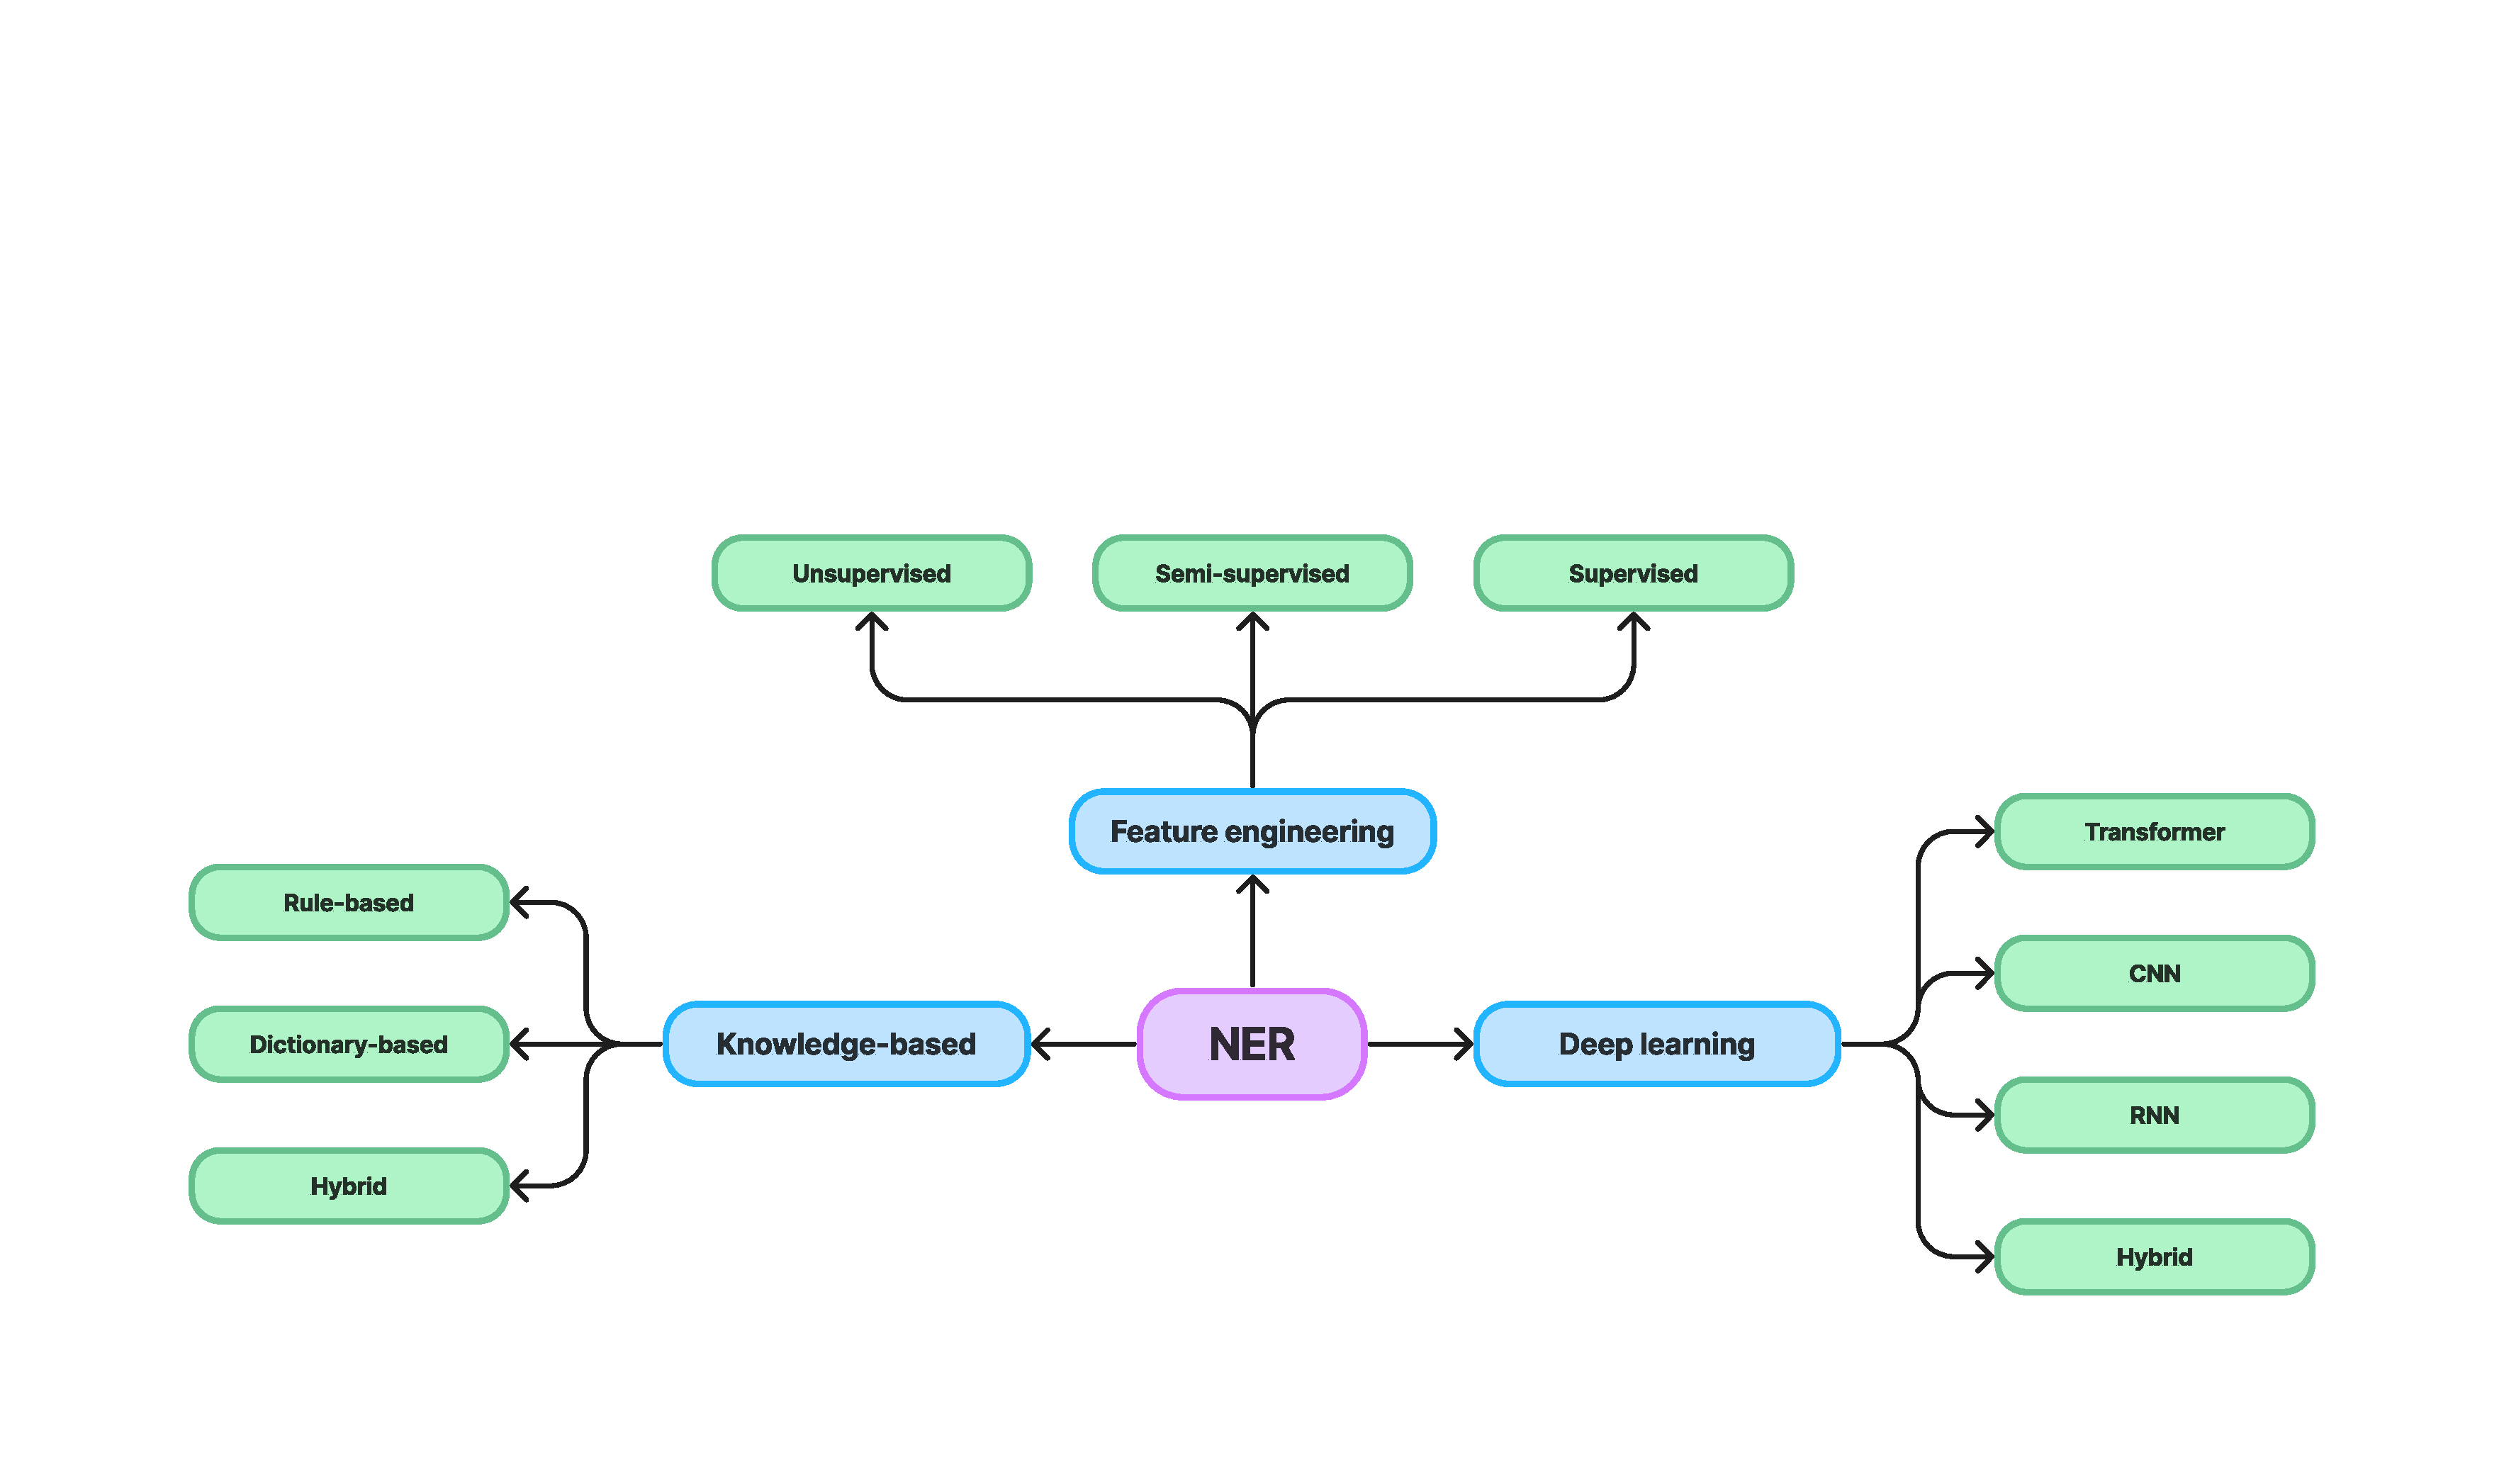
\includegraphics[width=\textwidth]{img/ner-methods.pdf}
    \caption{TODO: Named entity recognition main method approaches.}
    \label{fig:named-entity-recognition-methods}
\end{figure}

\subsubsection*{Knowledge-based}
\label{subsubsec:knowledge-based}
Knowledge-based approaches rely on predefined rules and dictionaries to identify entities. These rules and dictionaries, typically created by domain experts, recognise entities based on their characteristics. Rules can be given as regular expressions, denoting patterns to match character combinations in strings. Established on the chosen method, we separate this category into Rule-based and Dictionary-based or combine these approaches. The main advantage of knowledge-based approaches stems from their interpretability, as the rules and dictionaries can be easily understood and modified. Nevertheless, the principal disadvantage is frequent limitations to the entities in the manually created dictionaries and rules, as a result of which new entities cannot be recognised.

\subsubsection*{Feature engineering}
\label{subsubsec:feature-engineering}
Instead of manually creating a set of rules and a dictionary, feature engineering-based approaches, popularly identified as machine learning, use linguistic and statistical features to identify entities. These features are generally derived from the text and subsequently are used to train a machine learning model to recognise entities. The primary advantage of this approach is the ability to learn more about the data and discover patterns that may not be apparent at first. Additionally, their ability to recognise new entities differs from dictionaries in some cases. However, the main disadvantage is that these approaches require a large amount of labeled training data to be accurate.

Before exploring feature engineering-based methods in depth, we should clarify the data under discussion and the definition of labels. In the early introduction regarding named entity recognition, we referred to tags. These tags correspond to labels that serve as identifiers describing particular data that are consequently categorised according to the assigned label. To promote better comprehension, referring to the example illustrated in Figure \ref{fig:named-entity-recognition-theoretical-example}, we have textual data in which labels are assigned as outlined in the following Table \ref{table:text-data-with-labels}.
\\
\begin{table}[ht]
    \centering
    \caption{TODO: Textual data with according labels.}
    \label{table:text-data-with-labels}
    \begin{tabular}[t]{ll}
        \hline
        Data&Label\\
        \hline
        Tim Cook&\textbf{PERSON}\\
        Apple Inc.&\textbf{ORG}ANISATION\\
        June 8th, 2023&\textbf{DATE}\\
        \hline
    \end{tabular}
\end{table}

\begin{description}
    \item[Unsupervised learning] The unsupervised learning method discovers patterns of entity occurrence in raw and unlabeled data. Consequently, the individual entities are split into groups based on their characteristic properties. The absence of pre-labeled data by human intervention in the training phase causes no supervisor to guide the model with information about the labels in training data, hence unsupervised learning. A conventional method employed in this approach is clustering, such as K-means clustering \parencite{9072123kmeans}, which divides data\footnote{In our case, the data corresponds to tokens symbolising words.} into groups based on similarity or dissimilarity.
    \begin{figure}[H]
        \centering
        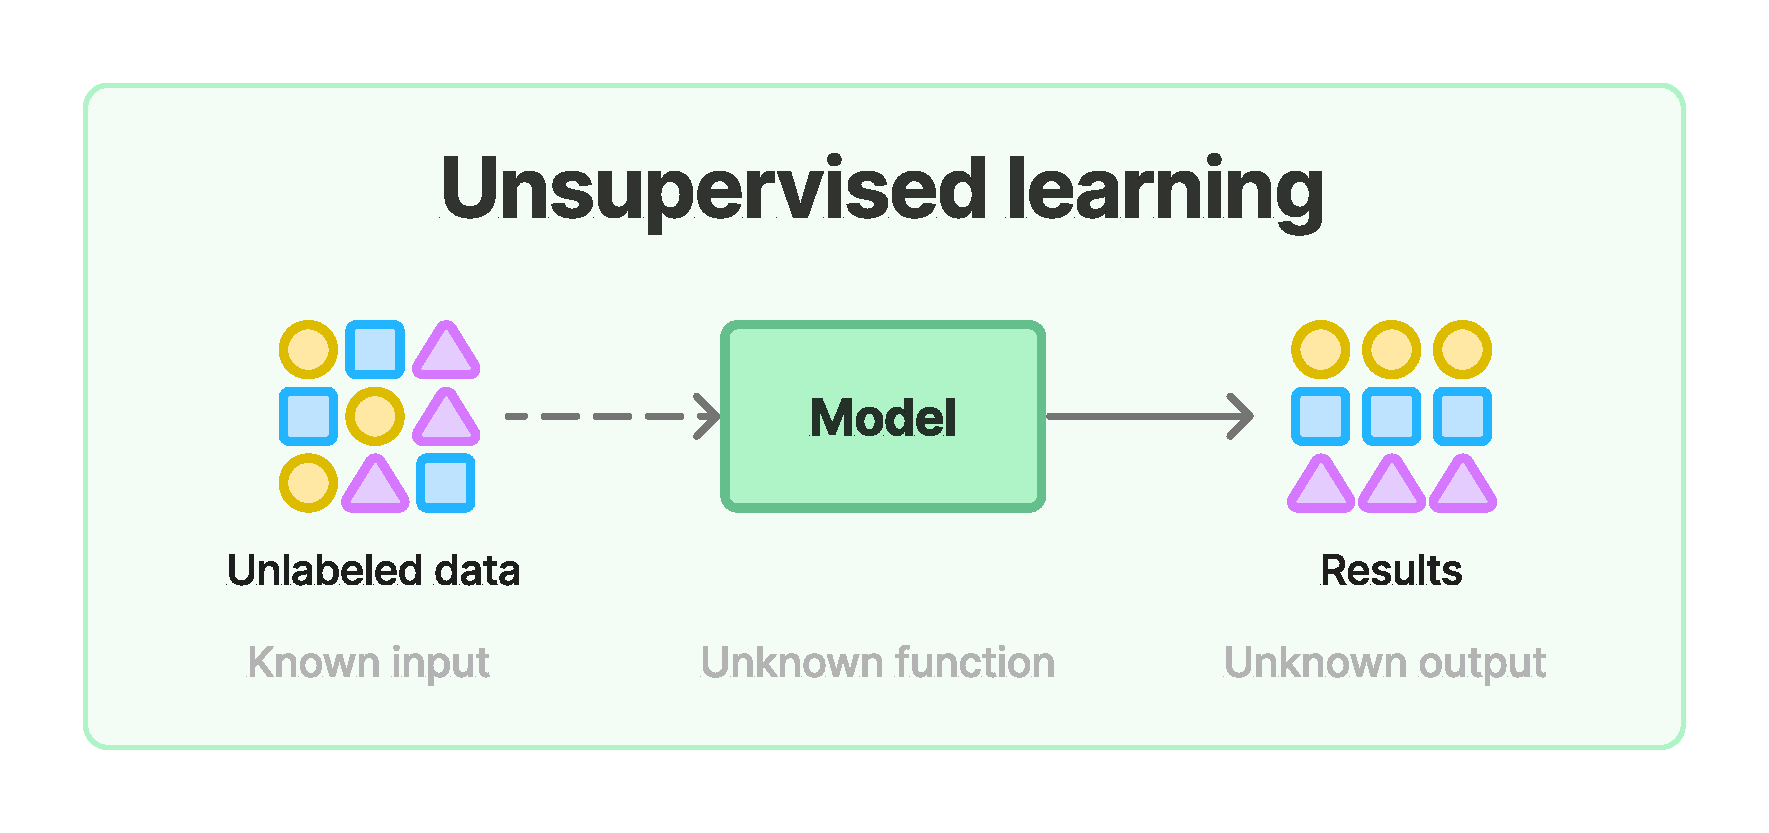
\includegraphics[width=0.6\textwidth]{img/unsupervised.pdf}
        \caption{TODO: Unsupervised learning.}
        \label{fig:unsupervised-learning}
    \end{figure}
    \item[Semi-supervised learning] The semi-supervised learning method combines labeled and unlabeled data, with the former comprising a slight portion of the dataset. As part of the classification training process, the unlabeled data learn the model's ability to generalise and represent the data in space using a statistical feature that better separates the classes. The algorithm aims to create the best decision boundary between classes based on a large amount of unlabeled data. Besides, the labeled data allows the model to determine the classification correctness for improvement, hence semi-supervised learning. Therefore, the model is partially supervised, hence semi-supervised learning. Semi-supervised learning is a preferred approach for model development because the labeled data is mainly expensive and time-consuming to acquire by requiring human intervention. In contrast, unlabeled data is more easily collectable.
    \begin{figure}[H]
        \centering
        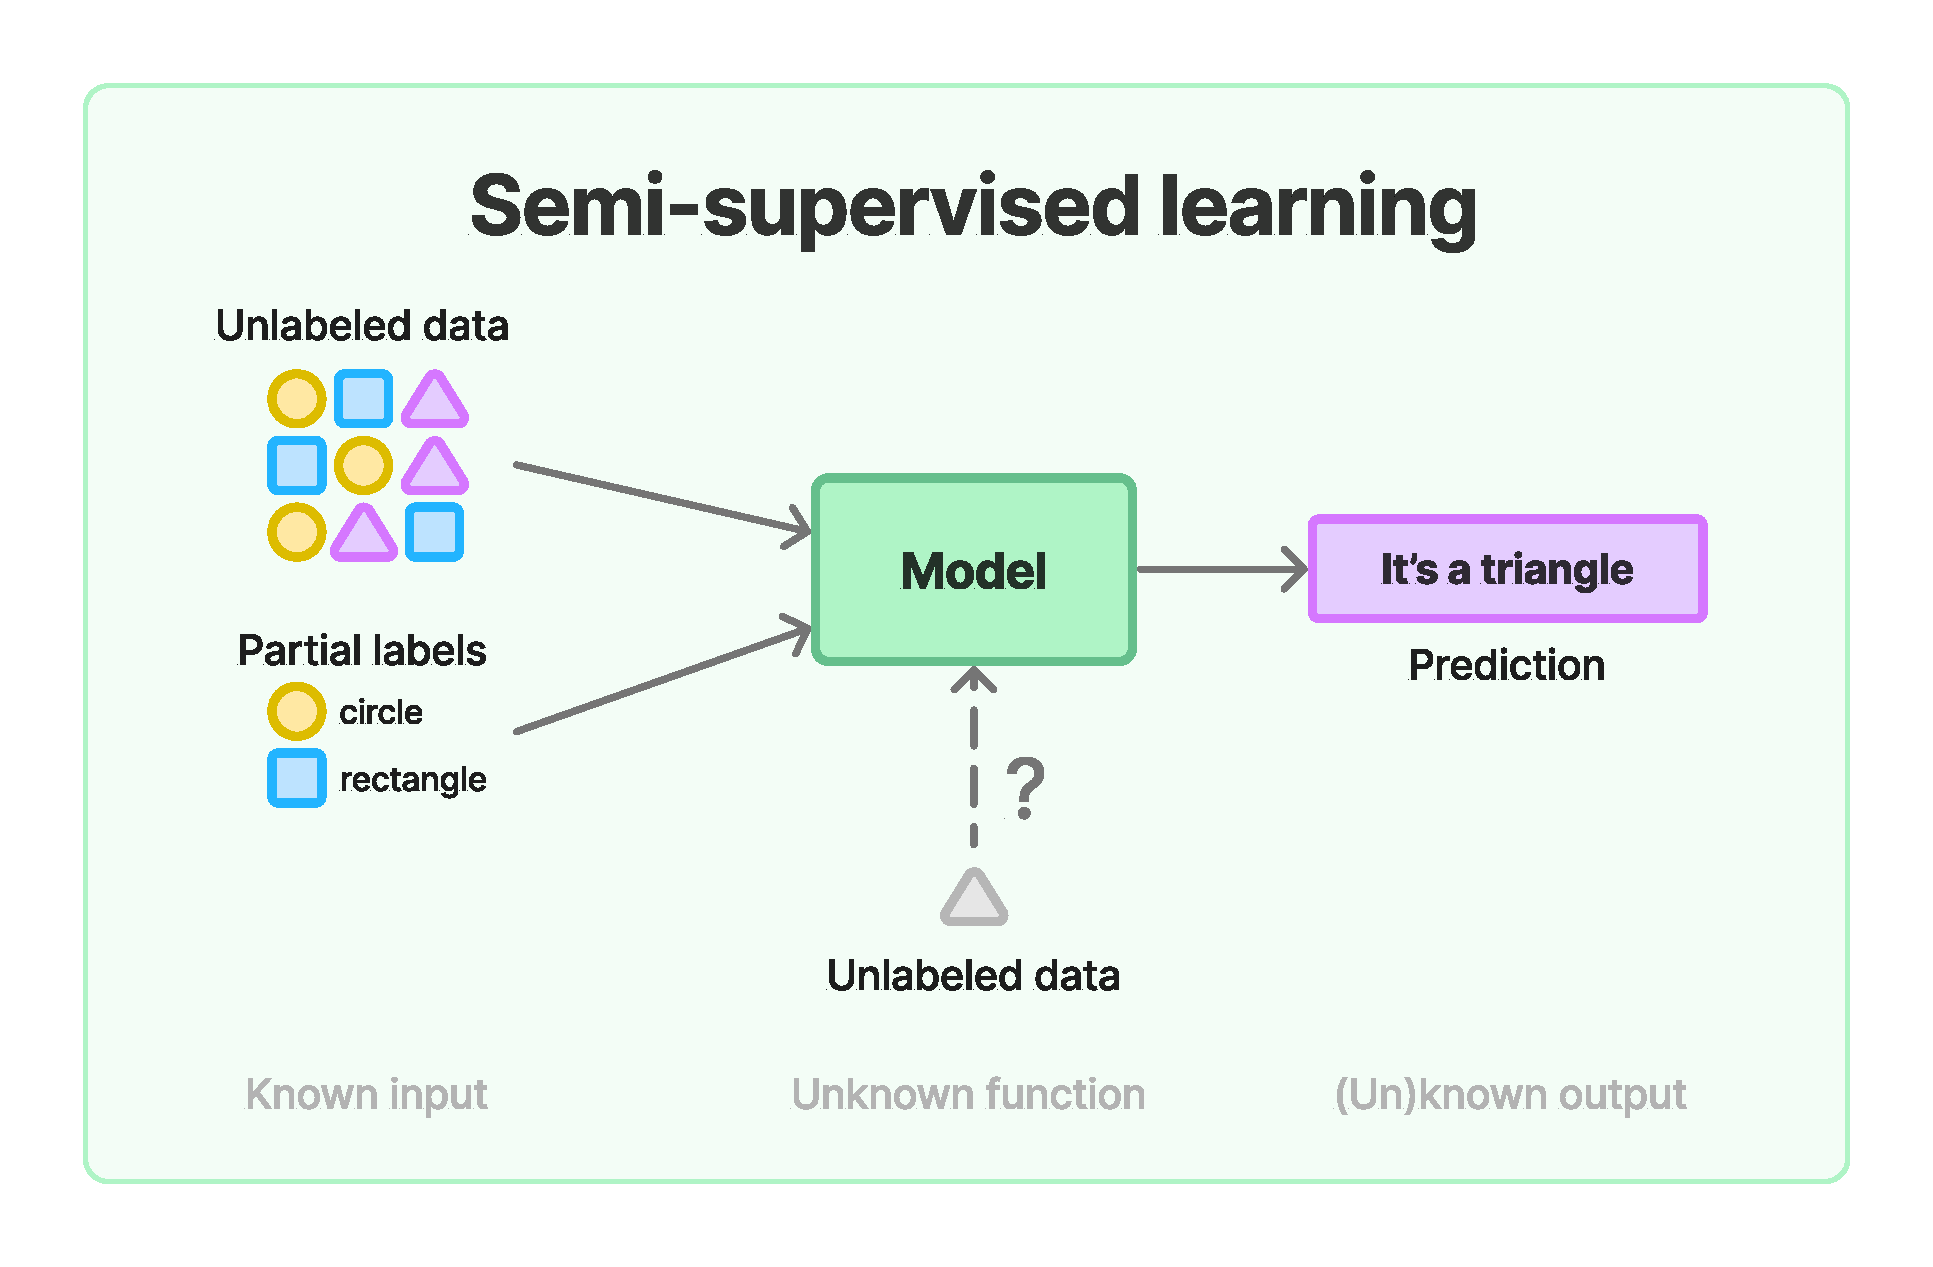
\includegraphics[width=0.6\textwidth]{img/semi-supervised.pdf}
        \caption{Semi-supervised learning.}
        \label{fig:semi-supervised-learning}
    \end{figure}
    Self-training, Co-training, and Multi-view learning are frequently employed subcategories of this learning method. Self-training involves using a small amount of labeled data and a more significant amount of unlabeled data, repeatedly training the model on labeled data and using it to predict labels for unlabeled data. Co-training uses multiple independent models that communicate and share information to improve performance. Multi-view learning combines information from different sources or representations of data, such as combining textual data with metadata.
    \item[Supervised learning] Unlike the semi-supervised learning method, the supervised learning approach exclusively utilises labeled data. Therefore, the training process is performed just on labeled data. We could perceive this approach as a function $f:~X~\mapsto~Y$, denoted as $f$, mapping input $X$ to output $Y$, where $X$ and $Y$ represent the input and output, respectively, known from the labeled data. Thus, as a supervisor guides the learning process, the model learns the most suitable way to map the input $X$ to the input $Y$. The principal contrast between fully and semi-supervised learning is that in the former case, learning is done only over labeled data and in the latter case on a combination with unlabeled data. The most common algorithms utilised in supervised learning for named entity recognition include statistical models like \acrfull{svm} \parencite{wang2005svm}, \acrfull{crf} \parencite{sutton2012crf}, \acrfull{me} \parencite{berger1996me}, and \acrfull{hmm} \parencite{EDDY1996361hmm}.
    \begin{figure}[H]
        \centering
        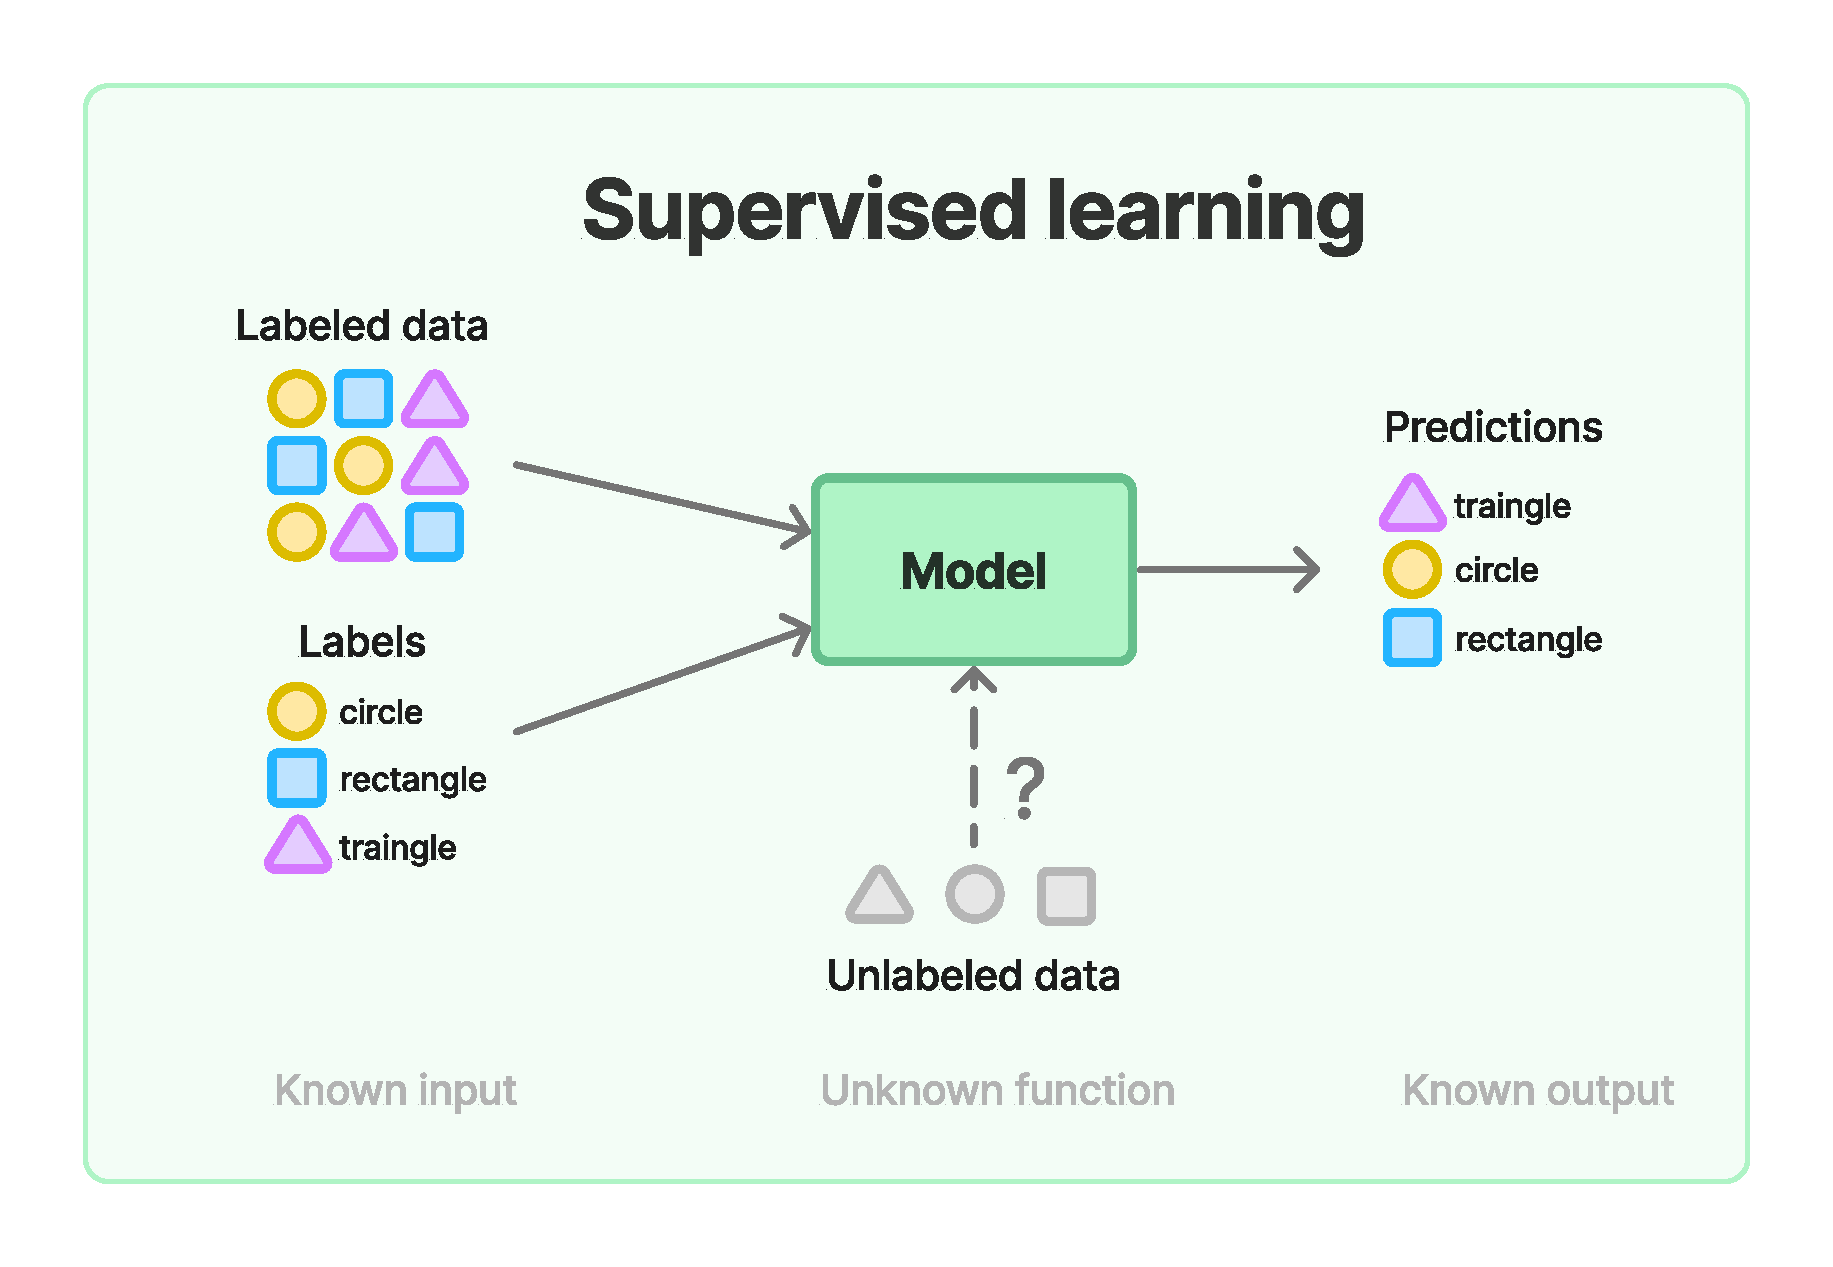
\includegraphics[width=0.6\textwidth]{img/supervised.pdf}
        \caption{TODO: Supervised learning.}
        \label{fig:supervised-learning}
    \end{figure}
\end{description}

\subsubsection*{Deep learning}
\label{subsubsec:deep-learning}
A given text could be extensive and contain many sentences or paragraphs mentioning entities in various forms. Therefore, deep learning comes into play due to its prowess in achieving better comprehension and learning contextual semantics. Its approaches overcome the primarily classification-focused methods introduced thus far, leading to state-of-the-art results in entity recognition. To enhance elucidation of the semantic context, methods' consideration of words occurring before and after words possess a role. The overarching structure of this approach's most commonly employed methods, such as \acrfull{rnn}, \acrfull{cnn}, and Transformer, is usually outlined into three fundamental stages: Data representation, Context encoding and Entity decoding.

\begin{enumerate}
    \item \textbf{Data representation} is the first stage, where the input data are transformed into a format suitable for the model. We convert words into vector space to operate effectively in the following stages and maximise the potential of computational power. Transformations, collectively referred to as word embeddings, encompass techniques like One-Hot Encoding, Word2Vec \parencite{mikolov2013word2vec}, and \acrfull{tf-idf} \parencite{AIZAWA200345tfidf}. 
    
    \begin{enumerate}
    \item \textbf{One-Hot Encoding} consists of a vector representation of a word with a $1$ occurring at its positional index in the dictionary and a $0$ otherwise. The dictionary can be thought of as a sentence that is a sequence of words in a row.

    \item \textbf{Word2Vec} projects words in a vector space that captures the meaning and relationships between other words. The projection into vector space allows the creation of a unique identification for each word in the corpus, with an emphasis on preserving syntactic and primarily semantic properties, making it possible to find synonyms after training on a large corpus.\todo{TODO?: Přidat zmínku o CBOW a Skip-gram?}

    \item \textbf{TF-IDF} as the name suggests, takes into account both the frequency of a word in a document and its occurrence across all documents in the corpus. Hence, a word's importance could be captured and then deduced whether it is an entity.
    \end{enumerate}

    Additional representations worth mentioning are FastText \parencite{joulin2016bagfasttext}, \acrfull{glove} \parencite{pennington-etal-2014-glove}, or \acrfull{elmo} \parencite{peters2018elmo}. While these data representations may also find application in feature engineering-based methods, they must be met in the context of deep learning for effective textual data utilisation in subsequent processes.
    \item \textbf{Context encoder} conveys the most crucial stage. Once we have the data in a suitable representation capable of capturing the context in which the word is found, the type of neural network selection to learn the model contextual semantics of the input data comes next.\todo{TODO!!! Následující část se mi nelíbí a pravděpodobně udělám ještě krátkou a ukázkovou sekci o Neural networks. Protože jsou využívány v Sentiment Analysis, Named Entity Recognition, Time Series Forecasting, Text Similarity} \textcolor{lightgray}{As the deep learning methods approach is introduced, it is good to mention that "deep" refers to the depth of the layers in the neural network. Thus, the neural networks mentioned afterwards contain more than one hidden layer of neutrons, a layer that is neither an input nor an output layer. The articles \parencites{ibm_neural_networks}{ibm_ai_ml_dl_nn} describe what neurons are and how deep neural networks differ from regular neural networks.}   
    \item \textbf{Entity decoder} is the final stage, where the model identifies and classifies entities in the text based on word representation and extracted context information. Entity decoding has two flavours based on the way the output of the previous stage is processed. 
    
    \begin{enumerate}
        \item \textbf{Classification models} such as softmax regression or multilayer perceptrons (MLP) can be used to assign labels to individual words in the text based on their representation and context. %upravit
        \item \textbf{Sequential models} such as recurrent neural networks (RNNs) or transformers are able to sequentially predict entity labels for individual words in a text given their context and relationships with other words. %upravit
    \end{enumerate}
\end{enumerate}

\begin{description}
    \item[RNN] 
    \item[CNN] 
    \item[Transformer]
    \begin{enumerate}
        \item \textbf{BERT}
    \end{enumerate}
    
    \item[Large language models]  
\end{description}

% There will be BERT mentioned
% TODO coding BERT https://www.analyticsvidhya.com/blog/2021/12/fine-tune-bert-model-for-sentiment-analysis-in-google-colab/

\section{Workflow of Entity-level Sentiment Analysis}
\label{sec:workflow-of-sentiment-analysis}
The sentiment analysis process can be divided into three main steps: data retrieval, preprocessing, and analysis. The following sections will discuss these steps in more detail.

\section{Time Series Forecasting Integration}
\label{sec:integration-with-time-series-forecasting-for-market-trends}
We will focus on integrating time series forecasting in the context of news.

\section{Text similarity}
\label{sec:text-similarity}

\todo{(Q-1.3) Zeptat se - Bude třeba úvod do stock marketu? - odpověď: ANO, bude třeba krátké intro.}

% Datasets:
% - https://huggingface.co/datasets/cc_news
% - https://arxiv.org/pdf/2305.12257.pdf